This chapter will present the results of the textural information extraction of the datasets and show the classification results obtained. It will be divided in three sections: the first section consists of the textures results for the TANDEM-X dataset and the land cover classification map obtained, the second section comprises the textures results for the SENTINEL-1 dataset and the land cover classification map created, and the last section presents the textures results for the CARABAS-II dataset and the results for the change detection algorithm that has been proposed.  

The texture extraction algorithm that was chosen for this work was the SADH method. This was decided based on the fact that it achieves similar textural information quality when compared to the GLCM method, but it is less time-consuming than the latter method --- in fact it was approximately four times faster to run SADH method than to run GLCM method for the same dataset.

\section{The TANDEM-X Results}
This section present the texture results for the TANDEM-X dataset using the SADH method and the subsequent land cover classification map that was created using the texture results.

\subsection{The TANDEM-X Texture Results}
From the TANDEM-X dataset it was chosen to extract the textural information of the volumetric coherence (also known as volumetric decorrelation) since it has been already shown that the volumetric coherence is the key information for creating forests maps using SAR data in the X-band \cite{Paolo,Rizzoli, Alberto}. For the TANDEM-X dataset the picture of the volumetric coherence can be seen in Figure \ref{fig:gamma_vol_tandemx}.

\begin{figure}[H]
    \centering
    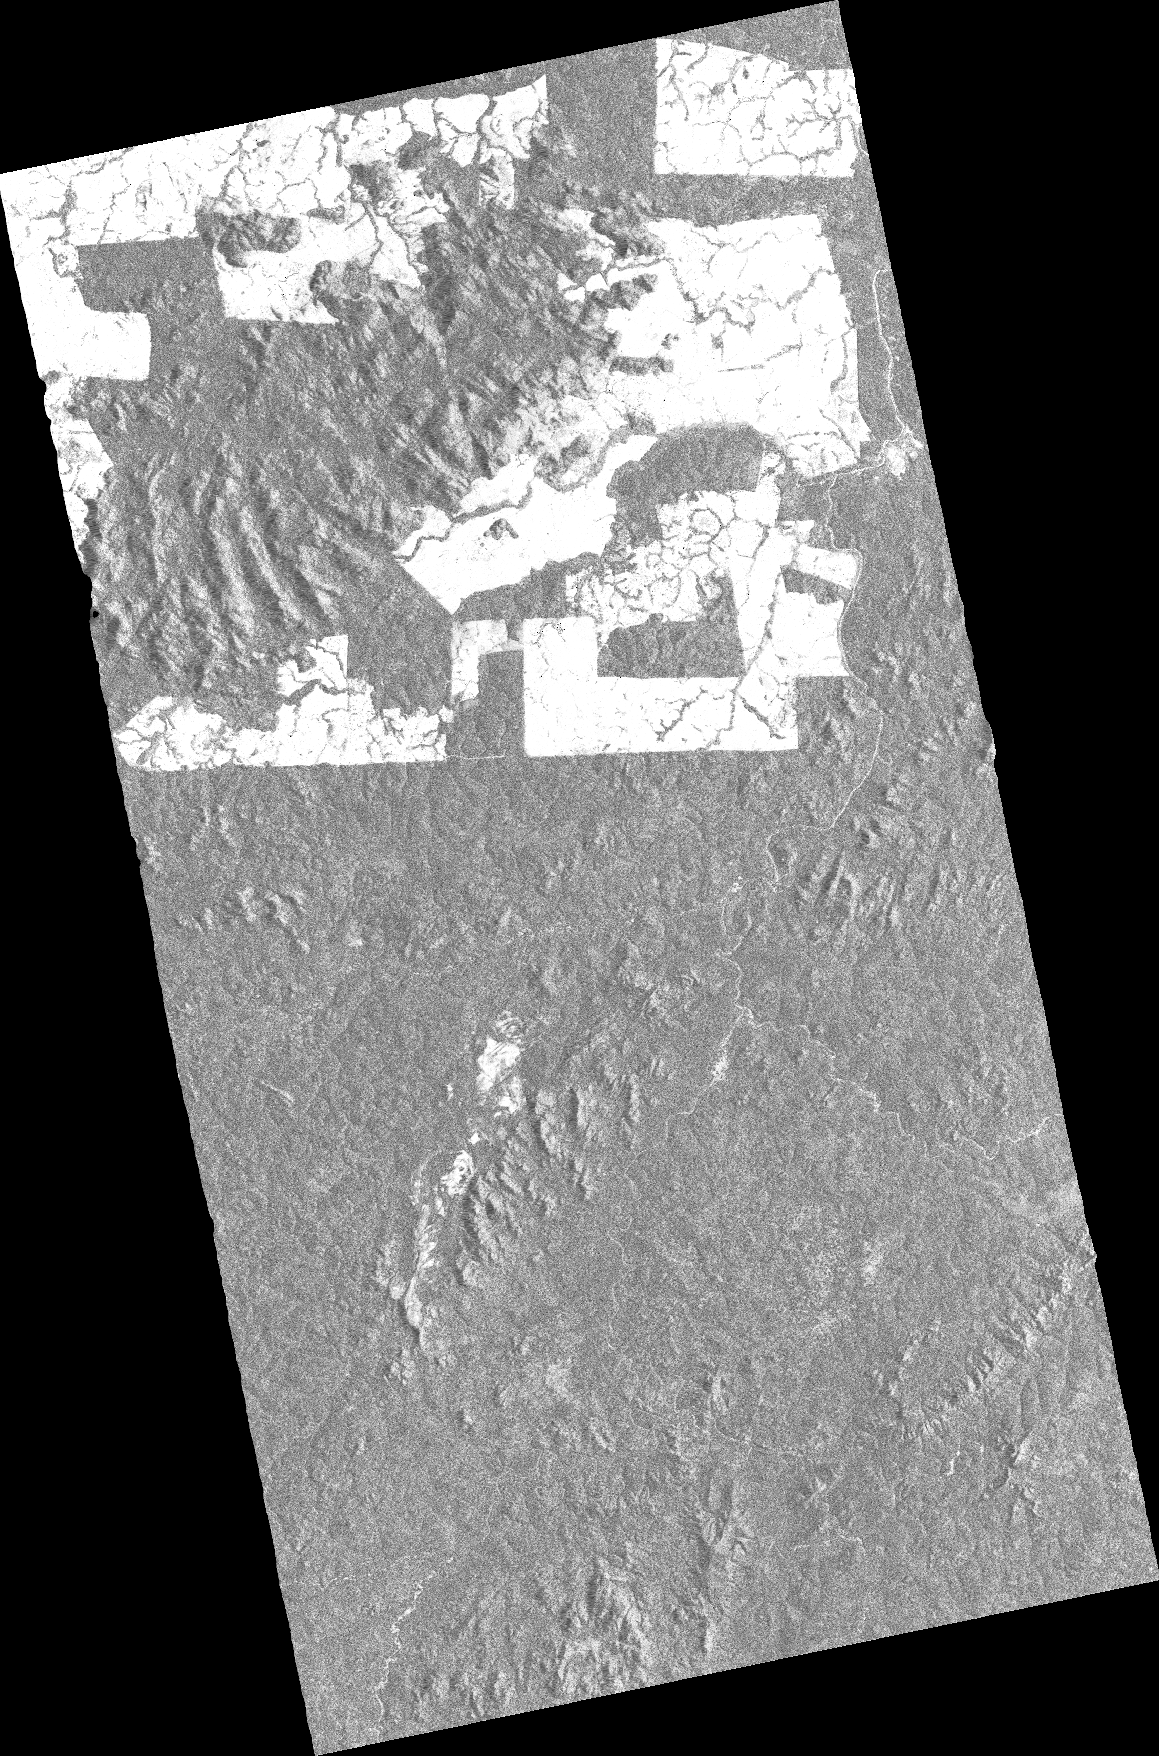
\includegraphics[width=0.4\linewidth]{Cap3-Results/coSSC_master_gamma_vol.png}
    \caption{Volumetric coherence acquisition of Amazon Rainforest area}
    \label{fig:gamma_vol_tandemx}
\end{figure}

Afterwards, each texture of the SADH method was extract for the area seen in Figure \ref{fig:gamma_vol_tandemx}. The image results for each image can be seen in Figure \ref{fig:tandemx_textures}.

In the next section it will be shown the land cover classification map that we were able to create with these additional textural information and how it compares to other classification maps already available.
\begin{figure}
    \centering
    \begin{subfigure}[b]{0.4\linewidth}
      \includegraphics[width=\linewidth]{Cap3-Results/sum_and_diff_textures/cluster_prominenceimage.png}
       \caption{Cluster Prominence Texture Image}
    \end{subfigure}
    \centering
    \begin{subfigure}[b]{0.4\linewidth}
      \includegraphics[width=\linewidth]{Cap3-Results/sum_and_diff_textures/cluster_shadeimage.png}
       \caption{Cluster Shade Texture Image}
    \end{subfigure}
    \centering
    \begin{subfigure}[b]{0.4\linewidth}
      \includegraphics[width=\linewidth]{Cap3-Results/sum_and_diff_textures/contrastimage.png}
       \caption{Contrast Texture Image}
    \end{subfigure}
    \centering
    \begin{subfigure}[b]{0.4\linewidth}
      \includegraphics[width=\linewidth]{Cap3-Results/sum_and_diff_textures/correlationimage.png}
       \caption{Correlation Texture Image}
    \end{subfigure}
  \end{figure}
  \newpage
  \begin{figure}[H]\ContinuedFloat
    \centering
    \begin{subfigure}[b]{0.4\linewidth}
      \includegraphics[width=\linewidth]{Cap3-Results/sum_and_diff_textures/energyimage.png}
       \caption{Energy Texture Image}
    \end{subfigure}
    \centering
    \begin{subfigure}[b]{0.4\linewidth}
      \includegraphics[width=\linewidth]{Cap3-Results/sum_and_diff_textures/entropyimage.png}
       \caption{Entropy Texture Image}
    \end{subfigure}
    \centering
    \begin{subfigure}[b]{0.4\linewidth}
      \includegraphics[width=\linewidth]{Cap3-Results/sum_and_diff_textures/homogeneityimage.png}
       \caption{ Homogeneity Texture Image}
    \end{subfigure}
    \centering
    \begin{subfigure}[b]{0.4\linewidth}
      \includegraphics[width=\linewidth]{Cap3-Results/sum_and_diff_textures/meanimage.png}
       \caption{Mean Texture Image}
    \end{subfigure}
  \end{figure}
  \newpage
  \begin{figure}[H]\ContinuedFloat
    \centering
    \begin{subfigure}[b]{0.4\linewidth}
      \includegraphics[width=\linewidth]{Cap3-Results/sum_and_diff_textures/varianceimage.png}
       \caption{Variance Texture Image}
    \end{subfigure}
    \caption{Sum and Difference Texture Images for the TANDEM-X Dataset.}
    \label{fig:tandemx_textures}
  \end{figure}

\subsection{The TANDEM-X Classification Map}
By combining the SADH information extracted for the TANDEM-X dataset with the original information that was available and using it as input to a Random Forest Algorithm we were able to generate a classification map for the Amazon Rainforest area. The random forest algorithm was trained using the reference map that was provided by DLR. Due to computational limitations not all textures were used, but just some of them. The textures chosen as input to the Random
Forest algorithms were: Cluster Shade, Cluster Prominence, Contrast, Variance. Besides
that, the coherence was also given as an input to the Random Forest Algorithm. The classification results are summarized in Table \ref{tab:tandemx_results}.

\begin{table}[H]
    \centering
    \begin{tabular}{ |c |c |}
     \hline
        Textures Combination & Error Probability \\ \hline \hline
        Cluster Prominence & 3.82\% \\ \hline
        Cluster Prominence/Coherence & 3.80\% \\ \hline
        Cluster Prominence/Variance & 4.17\% \\ \hline
        Cluster Prominence/Variance/Coherence & 4.70\% \\ \hline
        Cluster Shade & 1.33\% \\ \hline
        Cluster Shade/Cluster Prominence & 1.27\% \\ \hline
        Cluster Shade/Cluster Prominence/Coherence & 1.26\% \\ \hline
        Cluster Shade/Cluster Prominence/Variance & 1.26\% \\ \hline
        Cluster Shade/Cluster Prominence/Variance/Coherence & 1.28\% \\ \hline
        Cluster Shade/Coherence & 1.30\% \\ \hline
        Cluster Shade/Variance & 1.30\% \\ \hline
        Cluster Shade/Variance/Coherence & 1.30\% \\ \hline
        Coherence & 4.70\% \\ \hline
        Contrast & 21.13\% \\ \hline
        Contrast/Cluster Prominence & 4.42\% \\ \hline
        Contrast/Cluster Prominence/Coherence & 3.47\% \\ \hline
        Contrast/Cluster Prominence/Variance & 3.81\% \\ \hline
        Contrast/Cluster Prominence/Variance/Coherence & 3.47\% \\ \hline
        Contrast/Cluster Shade & 1.30\% \\ \hline
        Contrast/Cluster Shade/Cluster Prominence & 1.15\% \\ \hline
        Contrast/Cluster Shade/Cluster Prominence/Coherence & 1.47\% \\ \hline
        Contrast/Cluster Shade/Cluster Prominence/Variance & 1.52\% \\ \hline
        Contrast/Cluster Shade/Cluster Prominence/Variance/Coherence & 1.29\% \\ 
        Contrast/Cluster Shade/Coherence & 1.30\% \\ \hline
        Contrast/Cluster Shade/Variance & 1.30\% \\ \hline
        Contrast/Cluster Shade/Variance/Coherence & 1.40\% \\ \hline
        Contrast/Coherence & 5.18\% \\ \hline
        Contrast/Variance & 21.07\% \\ \hline
        Contrast/Variance/Coherence & 4.70\% \\ \hline
        Variance/Coherence & 4.70\% \\ \hline
        Variance & 46.78\% \\ \hline
    \end{tabular}
    \caption{Forest classification probability of error results with different textures combinations}
    \label{tab:tandemx_results}
\end{table}

From the Table \ref{tab:tandemx_results} it can be seen that it is possible to reduce the error probability from 4.70\% (using only the coherence image) down to 1.29\% by combining it with additional textural information such as: contrast, cluster shade, cluster prominence and variance.

Even though this improvement might seem surprising it is important to notice that the
coherence image used was a high quality image acquired with ideal conditions that yields a clear separation between the forest and deforested areas,
but normally the SARs acquisitions are not always this good for classification, specially if
it is not used a double satellite system like TANDEM-X (which has the advantage of not
having temporal decorrelation between images since they are taken at the same time). One must also keep in mind that the frequency band of operation and image resolution is a key factor for the quality of the final classification map, so one texture combination that works well in one system might not work as well as in another system.
On
the next section this method will be used on acquisitions that are not so suited to make a
classification in order to see the improvement that the textures can provide in non-ideal
conditions.

\section{The Sentinel-1 Results}
The Sentinel-1 dataset is not as well suited for making forest classification maps as the TANDEM-X dataset, so it will provide insightful information of how well texture methods can improve results when ideal conditions are not present. The Sentinel-1 dataset consists of image acquisitions over the Rondônia State and consists mainly of three different classes: forest areas, deforested areas, and artificial surfaces (i.e. man-made surfaces). 

As mentioned in chapter 3, the dataset consists of 12 image stacks, 8 of which were used for Random Forest training (which used PRODES classification reference map \cite{prodes}), and four were used for validation purposes. The results will be assessed in terms of overall accuracy, i.e. the number of pixels that were correctly classified divided by the number of pixels in the dataset. For explanations about different measures of accuracy such as average accuracy, precision, recall, F-score, the reader is referred to \cite{Book_ML}.

In order to try to generate the most accurate classification map possible, it will be used the state-of-the-art method for the creation of forest maps using Sentinel-1 data as described in \cite{Paolo}. The state-of-the-art method uses a combination of: radar brightness in the plane perpendicular to line of sight ($\gamma^0$ coefficient), incidence angle ($\theta_{inc}$), long-term coherence term ($\rho_{LT}$), and temporal decorrelation constant ($\tau$). This method will be run for the Sentinel-1 dataset without the textural information, and this method will also be run for the Sentinel-1 dataset with the additional textural information and overall accuracy results will be compared in order to access the impact that the texture information can make in the creation of classification maps. 

The texture results that were used were 18 in total: the 9 texture information that can be generated by SADH method using the displacement vector equal to 1 unit in the horizontal direction, and 9 other textures that can be generated by SADH method using the displacement vector equal to 1 unit in the vertical direction. As a reminder, the texture methods that can be created by SADH methods are: average, cluster shade, cluster prominence, contrast, correlation, energy, entropy, homogeneity, and variance.

The classification results for the 4 validation stacks of the Sentinel-1 dataset can be seen in Figure \ref{img:sentinel_results}.

\begin{figure}
    \centering
    \includegraphics{Cap3-Results/sentinel1-classificationresults.jpg}
    \caption{Comparison between the PRODES reference map (left) and the final results of the Random Forest algorithm using SADH textures (right). The white square identifies a region of interest in which the maps are clearly different.
    Such an area corresponds to the Pacaás Novos National Park.}
    \label{img:sentinel_results}
\end{figure}

The overall accuracy (OA) for each image stack can be seen in Table \ref{tab:sentinel_table_results}.

\begin{table}[H]
    \centering
    \begin{tabular}{ |c |c | c|}
     \hline
        Image Stack & Original OA & SADH OA\\ \hline \hline
        Stack 6 & 88.48 \% & 91.90 \% \\ \hline
        Stack 7 & 82.50 \% & 84.26 \% \\ \hline
        Stack 8 & 85.03 \% & 86.49 \% \\ \hline
        Stack 9 & 84.84 \% & 87.66 \% \\  \hline
    \end{tabular}
    \caption{Overall accuracy for the four images stack in Figure \ref{img:sentinel_results}.}
    \label{tab:sentinel_table_results}
\end{table}

\section{The CARABAS-II Results}





